\documentclass[11pt]{article}
%Fall 2022
% Some basic packages
\usepackage{standalone}[subpreambles=true]
\usepackage[utf8]{inputenc}
\usepackage[T1]{fontenc}
\usepackage{textcomp}
\usepackage[english]{babel}
\usepackage{url}
\usepackage{graphicx}
%\usepackage{quiver}
\usepackage{float}
\usepackage{enumitem}
\usepackage{lmodern}
\usepackage{comment}
\usepackage{hyperref}
\usepackage[usenames,svgnames,dvipsnames]{xcolor}
\usepackage[margin=1in]{geometry}
\usepackage{pdfpages}

\pdfminorversion=7

% Don't indent paragraphs, leave some space between them
\usepackage{parskip}

% Hide page number when page is empty
\usepackage{emptypage}
\usepackage{subcaption}
\usepackage{multicol}
\usepackage[b]{esvect}

% Math stuff
\usepackage{amsmath, amsfonts, mathtools, amsthm, amssymb}
\usepackage{bbm}
\usepackage{stmaryrd}
\allowdisplaybreaks

% Fancy script capitals
\usepackage{mathrsfs}
\usepackage{cancel}
% Bold math
\usepackage{bm}
% Some shortcuts
\newcommand{\rr}{\ensuremath{\mathbb{R}}}
\newcommand{\zz}{\ensuremath{\mathbb{Z}}}
\newcommand{\qq}{\ensuremath{\mathbb{Q}}}
\newcommand{\nn}{\ensuremath{\mathbb{N}}}
\newcommand{\ff}{\ensuremath{\mathbb{F}}}
\newcommand{\cc}{\ensuremath{\mathbb{C}}}
\newcommand{\ee}{\ensuremath{\mathbb{E}}}
\newcommand{\hh}{\ensuremath{\mathbb{H}}}
\renewcommand\O{\ensuremath{\emptyset}}
\newcommand{\norm}[1]{{\left\lVert{#1}\right\rVert}}
\newcommand{\dbracket}[1]{{\left\llbracket{#1}\right\rrbracket}}
\newcommand{\ve}[1]{{\bm{#1}}}
\newcommand\allbold[1]{{\boldmath\textbf{#1}}}
\DeclareMathOperator{\lcm}{lcm}
\DeclareMathOperator{\im}{im}
\DeclareMathOperator{\coim}{coim}
\DeclareMathOperator{\dom}{dom}
\DeclareMathOperator{\tr}{tr}
\DeclareMathOperator{\rank}{rank}
\DeclareMathOperator*{\var}{Var}
\DeclareMathOperator*{\ev}{E}
\DeclareMathOperator{\dg}{deg}
\DeclareMathOperator{\aff}{aff}
\DeclareMathOperator{\conv}{conv}
\DeclareMathOperator{\inte}{int}
\DeclareMathOperator*{\argmin}{argmin}
\DeclareMathOperator*{\argmax}{argmax}
\DeclareMathOperator{\graph}{graph}
\DeclareMathOperator{\sgn}{sgn}
\DeclareMathOperator*{\Rep}{Rep}
\DeclareMathOperator{\Proj}{Proj}
\DeclareMathOperator{\mat}{mat}
\DeclareMathOperator{\diag}{diag}
\DeclareMathOperator{\aut}{Aut}
\DeclareMathOperator{\gal}{Gal}
\DeclareMathOperator{\inn}{Inn}
\DeclareMathOperator{\edm}{End}
\DeclareMathOperator{\Hom}{Hom}
\DeclareMathOperator{\ext}{Ext}
\DeclareMathOperator{\tor}{Tor}
\DeclareMathOperator{\Span}{Span}
\DeclareMathOperator{\Stab}{Stab}
\DeclareMathOperator{\cont}{cont}
\DeclareMathOperator{\Ann}{Ann}
\DeclareMathOperator{\Div}{div}
\DeclareMathOperator{\curl}{curl}
\DeclareMathOperator{\nat}{Nat}
\DeclareMathOperator{\gr}{Gr}
\DeclareMathOperator{\vect}{Vect}
\DeclareMathOperator{\id}{id}
\DeclareMathOperator{\Mod}{Mod}
\DeclareMathOperator{\sign}{sign}
\DeclareMathOperator{\Surf}{Surf}
\DeclareMathOperator{\fcone}{fcone}
\DeclareMathOperator{\Rot}{Rot}
\DeclareMathOperator{\grad}{grad}
\DeclareMathOperator{\atan2}{atan2}
\DeclareMathOperator{\Ric}{Ric}
\let\vec\relax
\DeclareMathOperator{\vec}{vec}
\let\Re\relax
\DeclareMathOperator{\Re}{Re}
\let\Im\relax
\DeclareMathOperator{\Im}{Im}
% Put x \to \infty below \lim
\let\svlim\lim\def\lim{\svlim\limits}

%wide hat
\usepackage{scalerel,stackengine}
\stackMath
\newcommand*\wh[1]{%
\savestack{\tmpbox}{\stretchto{%
  \scaleto{%
    \scalerel*[\widthof{\ensuremath{#1}}]{\kern-.6pt\bigwedge\kern-.6pt}%
    {\rule[-\textheight/2]{1ex}{\textheight}}%WIDTH-LIMITED BIG WEDGE
  }{\textheight}% 
}{0.5ex}}%
\stackon[1pt]{#1}{\tmpbox}%
}
\parskip 1ex

%Make implies and impliedby shorter
\let\implies\Rightarrow
\let\impliedby\Leftarrow
\let\iff\Leftrightarrow
\let\epsilon\varepsilon

% Add \contra symbol to denote contradiction
\usepackage{stmaryrd} % for \lightning
\newcommand\contra{\scalebox{1.5}{$\lightning$}}

% \let\phi\varphi

% Command for short corrections
% Usage: 1+1=\correct{3}{2}

\definecolor{correct}{HTML}{009900}
\newcommand\correct[2]{\ensuremath{\:}{\color{red}{#1}}\ensuremath{\to }{\color{correct}{#2}}\ensuremath{\:}}
\newcommand\green[1]{{\color{correct}{#1}}}

% horizontal rule
\newcommand\hr{
    \noindent\rule[0.5ex]{\linewidth}{0.5pt}
}

% hide parts
\newcommand\hide[1]{}

% si unitx
\usepackage{siunitx}
\sisetup{locale = FR}

%allows pmatrix to stretch
\makeatletter
\renewcommand*\env@matrix[1][\arraystretch]{%
  \edef\arraystretch{#1}%
  \hskip -\arraycolsep
  \let\@ifnextchar\new@ifnextchar
  \array{*\c@MaxMatrixCols c}}
\makeatother

\renewcommand{\arraystretch}{0.8}

\renewcommand{\baselinestretch}{1.5}

\usepackage{graphics}
\usepackage{epstopdf}

\RequirePackage{hyperref}
%%
%% Add support for color in order to color the hyperlinks.
%% 
\hypersetup{
  colorlinks = true,
  urlcolor = blue,
  citecolor = blue
}
%%fakesection Links
\hypersetup{
    colorlinks,
    linkcolor={red!50!black},
    citecolor={green!50!black},
    urlcolor={blue!80!black}
}
%customization of cleveref
\RequirePackage[capitalize,nameinlink]{cleveref}[0.19]

% Per SIAM Style Manual, "section" should be lowercase
\crefname{section}{section}{sections}
\crefname{subsection}{subsection}{subsections}
\Crefname{section}{Section}{Sections}
\Crefname{subsection}{Subsection}{Subsections}

% Per SIAM Style Manual, "Figure" should be spelled out in references
\Crefname{figure}{Figure}{Figures}

% Per SIAM Style Manual, don't say equation in front on an equation.
\crefformat{equation}{\textup{#2(#1)#3}}
\crefrangeformat{equation}{\textup{#3(#1)#4--#5(#2)#6}}
\crefmultiformat{equation}{\textup{#2(#1)#3}}{ and \textup{#2(#1)#3}}
{, \textup{#2(#1)#3}}{, and \textup{#2(#1)#3}}
\crefrangemultiformat{equation}{\textup{#3(#1)#4--#5(#2)#6}}%
{ and \textup{#3(#1)#4--#5(#2)#6}}{, \textup{#3(#1)#4--#5(#2)#6}}{, and \textup{#3(#1)#4--#5(#2)#6}}

% But spell it out at the beginning of a sentence.
\Crefformat{equation}{#2Equation~\textup{(#1)}#3}
\Crefrangeformat{equation}{Equations~\textup{#3(#1)#4--#5(#2)#6}}
\Crefmultiformat{equation}{Equations~\textup{#2(#1)#3}}{ and \textup{#2(#1)#3}}
{, \textup{#2(#1)#3}}{, and \textup{#2(#1)#3}}
\Crefrangemultiformat{equation}{Equations~\textup{#3(#1)#4--#5(#2)#6}}%
{ and \textup{#3(#1)#4--#5(#2)#6}}{, \textup{#3(#1)#4--#5(#2)#6}}{, and \textup{#3(#1)#4--#5(#2)#6}}

% Make number non-italic in any environment.
\crefdefaultlabelformat{#2\textup{#1}#3}

% Environments
\makeatother
% For box around Definition, Theorem, \ldots
%%fakesection Theorems
\usepackage{thmtools}
\usepackage[framemethod=TikZ]{mdframed}

\theoremstyle{definition}
\mdfdefinestyle{mdbluebox}{%
	roundcorner = 10pt,
	linewidth=1pt,
	skipabove=12pt,
	innerbottommargin=9pt,
	skipbelow=2pt,
	nobreak=true,
	linecolor=blue,
	backgroundcolor=TealBlue!5,
}
\declaretheoremstyle[
	headfont=\sffamily\bfseries\color{MidnightBlue},
	mdframed={style=mdbluebox},
	headpunct={\\[3pt]},
	postheadspace={0pt}
]{thmbluebox}

\mdfdefinestyle{mdredbox}{%
	linewidth=0.5pt,
	skipabove=12pt,
	frametitleaboveskip=5pt,
	frametitlebelowskip=0pt,
	skipbelow=2pt,
	frametitlefont=\bfseries,
	innertopmargin=4pt,
	innerbottommargin=8pt,
	nobreak=false,
	linecolor=RawSienna,
	backgroundcolor=Salmon!5,
}
\declaretheoremstyle[
	headfont=\bfseries\color{RawSienna},
	mdframed={style=mdredbox},
	headpunct={\\[3pt]},
	postheadspace={0pt},
]{thmredbox}

\declaretheorem[%
style=thmbluebox,name=Theorem,numberwithin=section]{thm}
\declaretheorem[style=thmbluebox,name=Lemma,sibling=thm]{lem}
\declaretheorem[style=thmbluebox,name=Proposition,sibling=thm]{prop}
\declaretheorem[style=thmbluebox,name=Corollary,sibling=thm]{coro}
\declaretheorem[style=thmredbox,name=Example,sibling=thm]{eg}

\mdfdefinestyle{mdgreenbox}{%
	roundcorner = 10pt,
	linewidth=1pt,
	skipabove=12pt,
	innerbottommargin=9pt,
	skipbelow=2pt,
	nobreak=true,
	linecolor=ForestGreen,
	backgroundcolor=ForestGreen!5,
}

\declaretheoremstyle[
	headfont=\bfseries\sffamily\color{ForestGreen!70!black},
	bodyfont=\normalfont,
	spaceabove=2pt,
	spacebelow=1pt,
	mdframed={style=mdgreenbox},
	headpunct={ --- },
]{thmgreenbox}

\declaretheorem[style=thmgreenbox,name=Definition,sibling=thm]{defn}

\mdfdefinestyle{mdgreenboxsq}{%
	linewidth=1pt,
	skipabove=12pt,
	innerbottommargin=9pt,
	skipbelow=2pt,
	nobreak=true,
	linecolor=ForestGreen,
	backgroundcolor=ForestGreen!5,
}
\declaretheoremstyle[
	headfont=\bfseries\sffamily\color{ForestGreen!70!black},
	bodyfont=\normalfont,
	spaceabove=2pt,
	spacebelow=1pt,
	mdframed={style=mdgreenboxsq},
	headpunct={},
]{thmgreenboxsq}
\declaretheoremstyle[
	headfont=\bfseries\sffamily\color{ForestGreen!70!black},
	bodyfont=\normalfont,
	spaceabove=2pt,
	spacebelow=1pt,
	mdframed={style=mdgreenboxsq},
	headpunct={},
]{thmgreenboxsq*}

\mdfdefinestyle{mdblackbox}{%
	skipabove=8pt,
	linewidth=3pt,
	rightline=false,
	leftline=true,
	topline=false,
	bottomline=false,
	linecolor=black,
	backgroundcolor=RedViolet!5!gray!5,
}
\declaretheoremstyle[
	headfont=\bfseries,
	bodyfont=\normalfont\small,
	spaceabove=0pt,
	spacebelow=0pt,
	mdframed={style=mdblackbox}
]{thmblackbox}

\theoremstyle{plain}
\declaretheorem[name=Question,sibling=thm,style=thmblackbox]{ques}
\declaretheorem[name=Remark,sibling=thm,style=thmgreenboxsq]{remark}
\declaretheorem[name=Remark,sibling=thm,style=thmgreenboxsq*]{remark*}
\newtheorem{ass}[thm]{Assumptions}

\theoremstyle{definition}
\newtheorem*{problem}{Problem}
\newtheorem{claim}[thm]{Claim}
\theoremstyle{remark}
\newtheorem*{case}{Case}
\newtheorem*{notation}{Notation}
\newtheorem*{note}{Note}
\newtheorem*{motivation}{Motivation}
\newtheorem*{intuition}{Intuition}
\newtheorem*{conjecture}{Conjecture}

% Make section starts with 1 for report type
%\renewcommand\thesection{\arabic{section}}

% End example and intermezzo environments with a small diamond (just like proof
% environments end with a small square)
\usepackage{etoolbox}
\AtEndEnvironment{vb}{\null\hfill$\diamond$}%
\AtEndEnvironment{intermezzo}{\null\hfill$\diamond$}%
% \AtEndEnvironment{opmerking}{\null\hfill$\diamond$}%

% Fix some spacing
% http://tex.stackexchange.com/questions/22119/how-can-i-change-the-spacing-before-theorems-with-amsthm
\makeatletter
\def\thm@space@setup{%
  \thm@preskip=\parskip \thm@postskip=0pt
}

% Fix some stuff
% %http://tex.stackexchange.com/questions/76273/multiple-pdfs-with-page-group-included-in-a-single-page-warning
\pdfsuppresswarningpagegroup=1


% My name
\author{Jaden Wang}



\begin{document}
\centerline {\textsf{\textbf{\LARGE{Homework 6}}}}
\centerline {Jaden Wang}
\vspace{.15in}
\section{Lagrangian Mechanics}
Disclaimer: most derivatives and equations are computed by Mathematica. We have the following equantities where subscripts represent relating to (center of mass of) 1st or 2nd rod.
\begin{align*}
	\ve{ r}_1 = \frac{L}{2} \begin{pmatrix} \sin \theta_1 \\ -\cos \theta_1 \\0 \end{pmatrix} ,   \ \ve{ r}_2 = \begin{pmatrix} L \sin \theta_1 + \frac{L}{2} \sin \theta_2\\ -L \cos \theta_1 - \frac{L}{2} \cos \theta_2 \\0 \end{pmatrix}  \\
	\ve{ v}_1 = \frac{L}{2} \begin{pmatrix} \cos \theta_1 \dot{\theta}_1\\ \sin \theta_1 \dot{\theta}_1 \\0 \end{pmatrix}, \ \ve{ v}_2 = \begin{pmatrix} L \cos \theta_1 \dot{\theta}_1 + \frac{L}{2} \cos \theta_2 \dot{\theta}_2 \\L \sin \theta_1 \dot{\theta}_1 + \frac{L}{2} \sin \theta_2 \dot{\theta}_2\\0 \end{pmatrix} \\
	 \ve{ \omega}_1 = \begin{pmatrix} 0\\0\\ \dot{\theta}_1 \end{pmatrix} \ \ve{ \omega}_2 = \begin{pmatrix} 0\\0\\ \dot{\theta}_2 \end{pmatrix}, \  \mathcal{ I}_1 = \mathcal{ I}_2= \begin{pmatrix} \ve{ 0}_2 &0\\0& \frac{1}{12} m L^2 \end{pmatrix} 
\end{align*}
We can now compute the kinetic and potential energy of the system and therefore the Lagrangian and its derivatives:
\begin{align*}
	T &= \frac{1}{2} m (\ve{ v}_1 \cdot \ve{ v}_1+ \ve{ v}_2 \cdot \ve{ v}_2) + \frac{1}{2} \ve{ \omega}_1 ^{T} \mathcal{ I}_1 \ve{ \omega}_1 + \frac{1}{2} \ve{ \omega}_2^{T} \mathcal{ I}_2 \ve{ \omega}_2  \\
	&= \frac{1}{6} mL^2 \left( 4 \dot{\theta}_1^2 + 3 \cos ( \theta_1 - \theta_2) \dot{\theta}_1 \dot{\theta}_2 + \dot{\theta}_2^2 \right)  \\
	V &= -mg \frac{3L}{2}\cos \theta_1 -mg \frac{L}{2} \cos \theta_2 \\
	\mathscr{L} &:= T-V\\
	\frac{\partial \mathscr{L}}{\partial \theta_1} &= -\frac{1}{2} mL \left( L \sin(\theta_1 - \theta_2) \dot{\theta}_1 \dot{\theta}_2 + 3g \sin \theta_1  \right) \\
	\frac{\partial \mathscr{L}}{\partial \dot{\theta}_1} &= \frac{1}{6} mL^2 \left( 8 \dot{\theta}_1 + 3 \cos (\theta_1 - \theta_2) \dot{\theta}_2 \right)  \\
	\frac{d}{dt} \frac{\partial \mathscr{L}}{\partial \dot{\theta}_1} &= \frac{1}{6} mL^2 \left( 8 \ddot{\theta_1} -3 \sin(\theta_1 - \theta_2) (\dot{\theta}_1 -\dot{\theta}_2) \dot{\theta}_2 + 3 \cos(\theta_1 - \theta_2) \ddot{\theta}_2 \right)  \\
	\frac{\partial \mathscr{L}}{\partial \theta_2} &= \frac{1}{2} mL \left( L \sin(\theta_1 - \theta_2) \dot{\theta}_1 \dot{\theta}_2 - g \sin \theta_2  \right) \\
	\frac{\partial \mathscr{L}}{\partial \dot{\theta}_2} &= \frac{1}{6} mL^2 \left( 2 \dot{\theta}_2 + 3 \cos (\theta_1 - \theta_2) \dot{\theta}_1 \right)  \\
	\frac{d}{dt} \frac{\partial \mathscr{L}}{\partial \dot{\theta}_2} &= \frac{1}{6} mL^2 \left( 2 \ddot{\theta_2} -3 \sin(\theta_1 - \theta_2) (\dot{\theta}_1 -\dot{\theta}_2) \dot{\theta}_1 + 3 \cos(\theta_1 - \theta_2) \ddot{\theta}_1 \right)  
\end{align*}
Therefore, the Euler-Lagrange equations can be simplified as
\begin{align}
	mL \left( 9g \sin \theta_1 + 3L \sin (\theta_1 - \theta_2) \dot{\theta}_2^2 + 3L\cos (\theta_1 - \theta_2) \ddot{\theta}_2 + 8L \ddot{\theta}_1 \right) &= 0 \\
	mL \left( 3g \sin \theta_2 - 3L \sin (\theta_1 - \theta_2) \dot{\theta}_1^2 + 3L \cos (\theta_1 - \theta_2) \ddot{\theta}_1 + 2L \ddot{\theta}_2 \right) &= 0 .
\end{align}
\section{Newton-Euler}
Denote the gravity of two rods by $ \ve{ G}_1 = \ve{ G}_2 = \begin{pmatrix} 0\\-mg\\0 \end{pmatrix}$. Consider the 1st rod rotating about $ O$ which is fixed in the inertial frame. By parallel axis theorem, in the $ zz$ component we have $ \mathcal{ I}_1^{O} = \mathcal{ I}_1 + m\frac{L^2}{4} = \frac{1}{3} m L^2$ (and 0 elsewhere). We also have $ \ve{ r}_P = 2 \ve{ r}_1$. Let $ \ve{ F} = \begin{pmatrix} F_x \\ F_y \\0 \end{pmatrix}  $ be the tension force experienced by the 2nd rod at $ P$. Thus the tension force experienced by the 1st rod at $ P$ is $ -\ve{ F} $.  Then Euler's 2nd law about $ O$ states
\begin{align*}
	\frac{d \ve{ L}^{O} }{ dt} &= \ve{ M}_{net}^{O}  \\
	\mathcal{ I}_1^{O} \ddot{\theta_1} &= \ve{ r}_1 \times \ve{ G}_1 + \ve{ r}_P \times (-\ve{ F})  
\end{align*}
Only $ z$-components survive. Simplifying the equation yields
\begin{align}
	mL \left( 9g \sin \theta_1 + 3L \sin (\theta_1 - \theta_2) \dot{\theta}_2^2 + 3L\cos (\theta_1 - \theta_2) \ddot{\theta}_2 + 8L \ddot{\theta}_1 \right) = 0 .
\end{align}
We see that Equation 3 matches Equation 1!

Now let us consider the 2nd rod. By Euler's 1st law, we have
\begin{align*}
	m \ve{ \ddot{r}}_2 &= \ve{ F}_{net} = \ve{ G}_2  + \ve{ F}   \\
	\ve{ F} &= m \ve{ \ddot{r}}_2 - \ve{ G}_2   \\
	&= \begin{pmatrix} -\frac{1}{2}mL \left( 2 \sin \theta_1 \dot{\theta}_1^2 + \sin \theta_2 \dot{\theta}_2^2  - 2 \cos \theta_1 \ddot{\theta}_1 - \cos \theta_2 \ddot{\theta}_2 \right) \\ m \left( g + L \cos \theta_1 \dot{\theta}_1^2 + \frac{1}{2} L \cos\theta_2 \dot{\theta}_2^2  + L \sin \theta_1 \ddot{\theta}_1 + \frac{1}{2} L \sin\theta_2 \ddot{\theta}_2  \right) \\0 \end{pmatrix}  
\end{align*}
Euler's 2nd law on the 2nd rod about center of mass gives
\begin{align*}
	\frac{d \ve{ L}^{C_2} }{ dt} &= \ve{ M}_{net}^{C_2}  \\
	\mathcal{ I}_2 \ddot{\theta}_2 &= (\ve{ r}_p - \ve{ r}_2)  \times \ve{ F}  \\
	\begin{pmatrix} 0\\0\\ \frac{1}{12} mL^2 \ddot{\theta}_2 \end{pmatrix} &= \begin{pmatrix} -\frac{1}{2} L \sin \theta_2 \\ \frac{1}{2} L \cos \theta_2 \\0 \end{pmatrix} \times \ve{ F}  
\end{align*}
Only $ z$-components survive. Simplifying the equation yields
\begin{align}
	mL \left( 3g \sin \theta_2 - 3L \sin (\theta_1 - \theta_2) \dot{\theta}_1^2 + 3L \cos (\theta_1 - \theta_2) \ddot{\theta}_1 + 2L \ddot{\theta}_2 \right) = 0 .
\end{align}
We see that Equation 4 exactly matches Equation 2! Therefore, we have analytically shown that the two methods give equivalent equations of motion. Using $ m = 10 kg, L = 2m, g=9.8 m /s ^2, t_f = 20s$ and the initial conditions of $ \theta_1(0) = 1, \theta_2(0) = 0, \dot{\theta}(0) = 0, \dot{\theta}(0) =0$, we have the following plots:
~\begin{figure}[H]
	\centering
	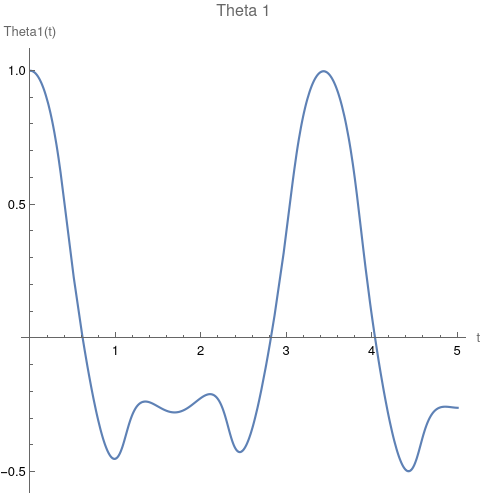
\includegraphics[width=0.49\textwidth]{./figures/hw6.1.png}
	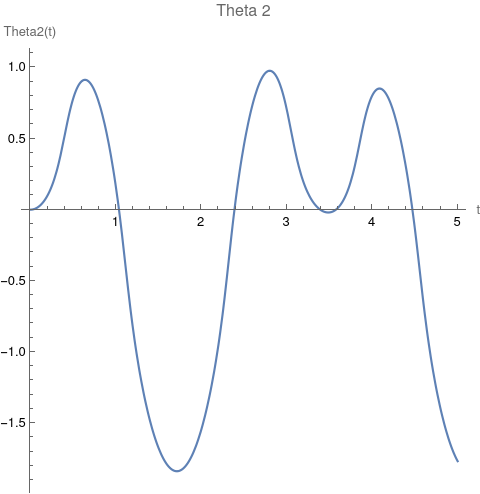
\includegraphics[width=0.49\textwidth]{./figures/hw6.2.png}
	\caption{Since the system start from being stationary and $ \theta_2$ being vertical, we expect $ \theta_1$ to drop and swing to the other side while $ \theta_2$ increasing initially. The plots match our expectations.}
\end{figure}
\end{document}
